\chapter{Specifikacija programske potpore}

\section{Funkcionalni zahtjevi}

\noindent \textbf{Dionici:}

\begin{packed_enum}
	
	\item Studenti
	\item Djelatnici studentskog centra			
	\item Razvojni tim
	
\end{packed_enum}

\noindent \textbf{Aktori i njihovi funkcionalni zahtjevi:}


\begin{packed_enum}
	\item  \underbar{Neregistrirani klijent (inicijator) može:}
	
	\begin{packed_enum}
		
		\item vidjeti predane oglase
		\item registrirati se u sustav, stvoriti novi korisnički račun i kasnije se prijaviti u sustav
		
	\end{packed_enum}
	
	\item  \underbar{Registrirani korisnik (student) (inicijator) može:}
	
	\begin{packed_enum}
		
		\item prijaviti se u sustav i odjaviti se iz sustava
		\item predati oglas za zamjenu sobe sa značajkama njegove sobe i željama sobe za zamjenu
		\item pregledati i uređivati vlastiti profil 
		\item vidjeti svoje aktivne i neaktivne oglase
		\item uređivati svoje aktivne oglase (promjeniti detalje oglasa ili ga učiniti neaktivnim)
		\item vidjeti oglase drugih korisinka te ih „lajkati“ ili označiti da se više ne prikazuje
		\item pregledati oglase koji odgovaraju njegovim kriterijima
		\item pregledati zaprimljene ponude za zamjenu
		\item potvrditi zamjenu soba
		
	\end{packed_enum}
		
	\item  \underbar{Djelatnik studentskog centra (sudionik) može:}
	
	\begin{packed_enum}
		
		\item vidjeti potvrđene (zaključane) zamjene između studenata
		\item označiti potvrđene zamjene koje je unio u sustav studentskog centra kao obavljene
		
	\end{packed_enum}
	
	\item  \underbar{Baza podataka (sudionik) može:}
	
	\begin{packed_enum}
		
		\item pohranjuje sve podatke o korisnicima
		\item pohranjuje sve podatke o predanim oglasima
		\item pohranjuje sve podatke o zamjenama
		
	\end{packed_enum}
\end{packed_enum}

\eject 



\subsection{Obrasci uporabe}


\subsubsection{Opis obrazaca uporabe}


\noindent \underbar{\textbf{UC1 - Pregledaj oglase}}
\begin{packed_item}
	
	\item \textbf{Glavni sudionik: } neregistrirani klijent, registrirani korisnik
	\item  \textbf{Cilj:} pregled ponude predanih oglasa
	\item  \textbf{Sudionici:} baza podataka
	\item  \textbf{Preduvjet:} -
	\item  \textbf{Opis osnovnog tijeka:}
	
	\item[] \begin{packed_enum}
		
		\item neregistrirani klijent/registrirani korisnik otvara aplikaciju
		\item sustav prikazuje predane oglase
		\item  neregistrirani klijent/registrirani korisnik listanjem aplikacije(„scrollanjem“) prema dolje može vidjeti još oglasa
		
	\end{packed_enum}
	
\end{packed_item}


\noindent \underbar{\textbf{UC2 - Registriraj korisnika}}
\begin{packed_item}
	
	\item \textbf{Glavni sudionik: } neregistrirani klijent
	\item  \textbf{Cilj:} stvaranje korisničkog računa koji omogućuje prijavu u sustav i predaju oglasa
	\item  \textbf{Sudionici:} baza podataka
	\item  \textbf{Preduvjet:} ispravna e-mail adresa i važeći JMBAG
	\item  \textbf{Opis osnovnog tijeka:}
	
	\item[] \begin{packed_enum}
		
		\item neregistrirani klijent u izborniku koji se nalazi u gornjem desnom kutu aplikacije odabire opciju za registraciju („Registriraj se“)
		\item sustav neregistriranog klijenta vodi na stranicu za registraciju na kojoj traži njegove korisničke podatke
		\item klijent unosi korisničko ime, e-mail adresu, JMBAG, ime i prezime te lozinku
		\item klijent odabire opciju za registraciju („Registriraj se“) koja se nalazi ispod unešenih podataka
		\item sustav prikazuje prikladnu poruku o uspješnoj registraciji 
		
	\end{packed_enum}
	
	\item  \textbf{Opis mogućih odstupanja:}
	
	\item[] \begin{packed_item}
		
		\item[3.a] odabrano korisničko ime je zauzeto ili je već postoji račun sa istom e-mail adresom
		\item[] \begin{packed_enum}
			
			\item sustav prikazuje prikladnu poruku  „Korisničko ime je zauzeto“ ili „Već postoji račun sa ovom e-mail adresom“
			
		\end{packed_enum}
	
		\item[3.b] korisnik nije unio sve potrebne podatke za registraciju (korisničko ime, e-mail adresu, JMBAG, ime i prezime ili lozinku)
		\item[] \begin{packed_enum}
			
			\item sustav prikazuje prikladnu poruku o potrebi za ispunjavanjem svih polja o korisničkim podacima
			
		\end{packed_enum}
		
	\end{packed_item}
\end{packed_item}


\noindent \underbar{\textbf{UC3 - Prijavi korisnika}}
\begin{packed_item}
	
	\item \textbf{Glavni sudionik: } registrirani korisnik (student ili djelatnik studentskog centra)
	\item  \textbf{Cilj:} pristupanje korisničkom sučelju, predaja oglasa
	\item  \textbf{Sudionici:} baza podataka
	\item  \textbf{Preduvjet:} registracija
	\item  \textbf{Opis osnovnog tijeka:}
	
	\item[] \begin{packed_enum}
		
		\item registrirani korisnik u izborniku u gornjem desnom kutu aplikacije odabire opciju za prijavu („Prijavi se“)
		\item sustav korisnika vodi na stranicu za prijavu na kojoj traži korisničko ime i lozinku te mu ispod podataka koje traži nudi gumb za prijavu („Prijavi se“)
		\item korisnik upisuje tražene podatke te odabire opciju za prijavu („Prijavi se“) 
		\item sustav obavještava korisnika o uspješnoj prijavi te mu dozvoljava pristup korisničkom sučelju
	
		
	\end{packed_enum}
	
	\item  \textbf{Opis mogućih odstupanja:}
	
	\item[] \begin{packed_item}
		
		\item[4.a] neispravan unos korisničkog imena ili  lozinke
		\item[] \begin{packed_enum}
			
			\item sustav obavještava korisnika o neuspjeloj prijavi te mu nudi ponovni pokušaj
			
		\end{packed_enum}

	\end{packed_item}
\end{packed_item}



	\noindent \underbar{\textbf{UC4 - Odjavi korisnika}}
	\begin{packed_item}
		
		\item \textbf{Glavni sudionik: } registrirani korisnik (student ili djelatnik studentskog centra)
		\item  \textbf{Cilj:} odjava iz korisničkog sučelja
		\item  \textbf{Sudionici:} baza podataka
		\item  \textbf{Preduvjet:} registracija, prijava
		\item  \textbf{Opis osnovnog tijeka:}
		
		\item[] \begin{packed_enum}
			
			\item registrirani korisnik u izborniku u gornjem desnom kutu aplikacije odabire opciju za odjavljivanje („Odjava“)	
			\item sustav odjavljuje korisnika te ga vodi na početnu stranicu gdje može vidjeti oglase svih korisnika, a u gornjem desnom kutu aplikacije, u izborniku ima opcije  „Početna“, „Prijavi se“ i „Registriraj se“ 
		\end{packed_enum}
	
	\end{packed_item}

\noindent \underbar{\textbf{UC5 - Predaj oglas}}
\begin{packed_item}
	
	\item \textbf{Glavni sudionik: } registrirani korisnik
	\item  \textbf{Cilj:} predaja vlastitog oglasa u sustav
	\item  \textbf{Sudionici:} baza podataka
	\item  \textbf{Preduvjet:} registracija, prijava
	\item  \textbf{Opis osnovnog tijeka:}
	
	\item[] \begin{packed_enum}
		
		\item registrirani korisnik odabire opciju za pregled vlastith oglasa („Moji oglasi“) koja se nalazi u izborniku u gornjem desnom kutu aplikacije 
		\item sustav vodi korisnika na stranicu na kojoj se nalaze svi neaktivni oglasi korisnika te mu na gornjem dijelu ekrana nudi opciju za stvaranje novog oglasa
		\item korisnik odabire opciju za stvaranje novog oglasa
		\item sustav vodi korisnika na stranicu za predaju novog oglasa, na kojoj od njega traži značajke (grad, dom, paviljon, kategorija sobe, kat, najbliža menza) njegove sobe u domu (ispunjavanje svih podataka o sobi koju korisnik nudi je obavezno)
		\item korisnik ispunjuje tražene podatke te odabire opciju „Predaj oglas“ koja se nalazi ispod kućica za upis traženih podataka
		\item sustav korisniku ispisuje poruku o uspješnoj predaji oglasa te ga vraća na stranicu „Moji oglasi“
		\item ukoliko je korisnik imao aktivan oglas prilikom predaje novog oglasa, on predajom novog oglasa automatski postaje neaktivan jer jedan korisnik može imati najviše jedan aktivan oglas istovremeno
		\item korisnik zatim vidi svoj novi aktivan oglas i sve neaktivne oglase
		
	\end{packed_enum}


\item  \textbf{Opis mogućih odstupanja:}

\item[] \begin{packed_item}
	
	\item[6.a] korisnik nije unio sve obavezne podatke (grad, dom, paviljon, kategorija sobe, kat, najbliža menza) o sobi koju nudi
	\item[] \begin{packed_enum}
		
		\item korisnik ne može predati oglas dok ne ispuni sve obavezne podatke
		\item sustav ispisuje odgovarajuću obavijest
		
	\end{packed_enum}
	
\end{packed_item}
	
\end{packed_item}



\noindent \underbar{\textbf{UC6 - Pregledaj vlastite oglase}}
\begin{packed_item}
	
	\item \textbf{Glavni sudionik: } registrirani korisnik
	\item  \textbf{Cilj:} pregled vlastitih predanih oglasa
	\item  \textbf{Sudionici:} baza podataka
	\item  \textbf{Preduvjet:} registracija, prijava
	\item  \textbf{Opis osnovnog tijeka:}
	
	\item[] \begin{packed_enum}
		
		\item registrirani korisnik odabire opciju za pregled vlastith oglasa koja se nalazi u izborniku u gornjem desnom kutu aplikacije („Moji oglasi“)
		\item sustav vodi korisnika na stranicu na kojoj se nalaze svi neaktivni oglasi korisnika, aktivan oglas (ako takav postoji) te opcija za stvaranje novog oglasa
		\item ukoliko korisnik ima više oglasa može ih pogledati listanjem aplikacije („scrollanjem“) prema dolje
		\item korisnik se može vratiti na početnu stranicu klikom na „Početna“ u izborniku u gornjem desnom kutu aplikacije
		
		
	\end{packed_enum}
	
	\item  \textbf{Opis mogućih odstupanja:}
	
	\item[] \begin{packed_item}
		
		\item[2.a] nepostojanje oglasa
		\item[] \begin{packed_enum}
			
			\item sustav ispisuje prikladnu poruku o nepostojanju oglasa
			\item sustav nudi korisniku da stvori oglas
			
		\end{packed_enum}
		
	\end{packed_item}
	
\end{packed_item}


\noindent \underbar{\textbf{UC7 - Uredi oglas}}
\begin{packed_item}
	
	\item \textbf{Glavni sudionik: } registrirani korisnik
	\item  \textbf{Cilj:} promjena detalja oglasa
	\item  \textbf{Sudionici:} baza podataka
	\item  \textbf{Preduvjet:} registracija, prijava, postojanje oglasa
	\item  \textbf{Opis osnovnog tijeka:}
	
	\item[] \begin{packed_enum}
		
		\item registrirani korisnik odabire opciju za pregled vlastith oglasa koja se nalazi u izborniku u gornjem desnom kutu aplikacije („Moji oglasi“)
		\item sustav vodi korisnika na stranicu na kojoj se nalazi aktivan oglas ukoliko postoji i svi neaktivni oglasi korisnika
		\item korisnik odabire opciju za uređivanje oglasa u donjem desnom kutu oglasa kojeg želi urediti („uredi“)
		\item sustav korisnika vodi na stranicu „Uredi oglas“ na kojoj korisnik može promijeniti bilo koji detalj vezan za oglas
		\item korisnik po želji mijenja podatke o oglasu
		\item sustav na dnu stranice za uređivanje oglasa nudi korisniku opcije „Spremi promjene“
		\item korisnik odabirom opcije „Spremi promjene“ mijenja detalje oglasa
		\item nakon odabira opcije „Spremi promjene“ ili odabira izlaska iz stranice za uređivanje oglasa (X u gornjem desnom kutu), sustav vraća korisnika na stranicu „Moji oglasi“ gdje se sada nalazi izmjenjen oglas(ukoliko je korisnik odabrao opciju „Spremi promjene“), ili oglas koji je isti kao i prije (ukoliko je korisnik odabrao izaći bez promjena)
		\item korisnik se može vratiti na početnu stranicu klikom na „Početna“ u izborniku u gornjem desnom kutu aplikacije
		
	\end{packed_enum}
	
\end{packed_item}


	

\noindent \underbar{\textbf{UC8 - Uredi profil}}
\begin{packed_item}
	
	\item \textbf{Glavni sudionik: } registrirani korisnik (student ili djelatnik studentskog centra)
	\item  \textbf{Cilj:}  promjena detalja profila
	\item  \textbf{Sudionici:} baza podataka
	\item  \textbf{Preduvjet:} registracija, prijava
	\item  \textbf{Opis osnovnog tijeka:}
	
	\item[] \begin{packed_enum}
		
		\item korisnik odabire opciju „Uredi profil“ u izborniku u gornjem desnom kutu aplikacije 
		\item sustav prikazuje korisniku njegove korisničke podatke (korisničko ime, ime i prezime, JMBAG, e-mail adresu)
		\item korisnik odabire opciju „uredi“ koja se nalazi ispod svih podataka
		\item sustav omogućuje korisniku promjenu bilo kojeg od podataka ili promjenu lozinke 
		\item korisnik mijenja željene podatke
		\item sustav korisniku nudi opcije „Ažuriraj podatke“ i „Ažuriraj lozinku“
		\item korisnik odabire jednu od ponuđenih opcija
		\item sustav ponovno prikazuje korisniku njegove korisničke podatke koji su izmjenjeni ili isti(ukoliko je mijenjao lozinku), ovisno o korisnikovom ranijem odabiru
		\item korisnik se može vratiti na početnu stranicu klikom na „Početna“ u izborniku u gornjem desnom kutu aplikacije
			
	\end{packed_enum}
	
\end{packed_item}



\noindent \underbar{\textbf{UC9 - Reagiraj na oglas}}
\begin{packed_item}
	
	\item \textbf{Glavni sudionik: } registrirani korisnik
	\item  \textbf{Cilj:}  izraziti želju za zamjenom sobe s korisnikom koji je dao oglas ili spriječiti ponovno pojavljivanje određenog oglasa
	\item  \textbf{Sudionici:} baza podataka
	\item  \textbf{Preduvjet:} registracija, prijava, postojanje aktivnog oglasa
	\item  \textbf{Opis osnovnog tijeka:}
	
	\item[] \begin{packed_enum}
		
		\item registrirani korisnik želi reagirati na određeni oglas
		\item korisnik odabire jednu od opcija za reagiranje na oglas koje su prikazane simbolom 1, 2 ili 3 srca, tj. kantom za smeće
		\item opcije koje su prikazane simbolima srca označuju stupanj sviđanja (1-malo, 3-jako), dok opcija koja je prikazana simbolom kante za smeće označuje da korisnik ne želi da mu se taj oglas više prikazuje
		\item ako je oglas „lajkan“ sustav šalje e-mail korisniku čiji je oglas „lajkan“ koji sadrži poruku „Imate nove kandidate za zamjenu sobe u domu!“ te link na stranicu „Dobiveni lajkovi“ koja se nalazi u izborniku u gornjem desnom kutu aplikacije gdje korisnik može vidjeti aktivne oglase svih korisnika koji su „lajkali“ njegov aktivan oglas
			
	\end{packed_enum}

\end{packed_item}

	

\noindent \underbar{\textbf{UC10 - Pregledaj oglase koji odgovaraju kriterijima}}
\begin{packed_item}
	
	\item \textbf{Glavni sudionik: } registrirani korisnik
	\item  \textbf{Cilj:}  pronalazak sobe za zamjenu
	\item  \textbf{Sudionici:} baza podataka
	\item  \textbf{Preduvjet:} registracija, prijava, postojanje aktivnog oglasa
	\item  \textbf{Opis osnovnog tijeka:}
	
	\item[] \begin{packed_enum}
		
		\item korisnik na početnoj stranici odabire opciju „Filtracija oglasa“
		\item korisnik unosi podatke o željenoj sobi te odabire opciju „Pretraži“
		\item korisnik također može odabrati i opcije „Spremi filter“ koja mu omogućuje spremanje unešenog filtera i „Prikaži spremljene filtere“ koja mu omogućuje prikaz do sada spremljenih oglasa
		\item korisnik može reagirati na bilo koji od oglasa koji su dobiveni filtriranjem
		
	\end{packed_enum}

\end{packed_item}



\noindent \underbar{\textbf{UC11 - Pregledaj zaprimljene ponude za zamjenu}}
\begin{packed_item}
	
	\item \textbf{Glavni sudionik: } registrirani korisnik
	\item  \textbf{Cilj:}  pregled oglasa onih korisnika koji žele zamjeniti sobu sa korisnikom
	\item  \textbf{Sudionici:} baza podataka
	\item  \textbf{Preduvjet:} registracija, prijava, postojanje aktivnog oglasa
	\item  \textbf{Opis osnovnog tijeka:}
	
	\item[] \begin{packed_enum}
		
		\item korisnik odabire opciju „Dobiveni lajkovi" koja se nalazi u izborniku u gornjem desnom kutu aplikacije
		\item sustav vodi korisnika na stranicu na kojoj mu prikazuje oglase studenata koji su „lajkali“ njegov oglas 
		\item korisnik pregledava zaprimljene ponude za zamjenu te po želji reagira na njih
		
	\end{packed_enum}
	
	\item  \textbf{Opis mogućih odstupanja:}
	
	\item[] \begin{packed_item}
		
		\item[2.a] nema novih kandidata za zamjenu
		\item[] \begin{packed_enum}
			
			\item sustav ispisuje prikladnu poruku
			
		\end{packed_enum}
	\end{packed_item}
\end{packed_item}



\noindent \underbar{\textbf{UC12 - Potvrdi zamjenu}}
\begin{packed_item}
	
	\item \textbf{Glavni sudionik: } registrirani korisnik
	\item  \textbf{Cilj:}  konačni odabir zamjene soba
	\item  \textbf{Sudionici:} baza podataka
	\item  \textbf{Preduvjet:} registracija, prijava, postojanje aktivnog oglasa, međusobno „lajkanje“ oglasa dvoje korisnika
	\item  \textbf{Opis osnovnog tijeka:}
	
	\item[] \begin{packed_enum}
		
		\item korisnik odlazi na stranicu „Moguće zamjene“ koja se nalazi u izborniku u gornjem desnom kutu aplikacije
		\item korisnik dolazi na stranicu na kojoj se prikazuje oglas ponuđene sobe za potvrdu zamjene (oglas može ponovno pogledati) te se ispod njega nalaze opcije „Potvrdi zamjenu“ i „Odbij zamjenu“
		\item korisnik potvrđuje zamjenu odabirom opcije „Potvrdi zamjenu“ ili ju odbija odabirom opcije „Odbij zamjenu“
		\item ukoliko svi korisnici uključeni u zamjenu potvrde zamjenu, djelatnik studentskog centra dobiva podatke o zamjeni, a ukoliko barem jedan od korisnika uključenih u zamjenu odbije zamjenu, svi uključeni u zamjenu dobivaju e-mail o neuspjelom ostvarenju zamjene
		
	\end{packed_enum}
	
	\item  \textbf{Opis mogućih odstupanja:}
	
	\item[] \begin{packed_item}
		
		\item[3.a] svi korisnici uključeni u zamjenu nisu potvrdili niti odbili zamjenu
		\item[] \begin{packed_enum}
			
			\item sustav nakon 7 dana briše ponudu za potvrdu ili odbijanje zamjene te se ona automatski smatra neostvarenom
			\item sustav šalje svim korisnicima uključenim u zamjenu e-mail o neuspjelom ostvarenju zamjene 
			
		\end{packed_enum}

		\item[3.b] jedan ili više korisnika uključenih u zamjenu je učinio svoj oglas neaktivnim, a drugi korisnik (korisnici) su potvrdili zamjenu
		\item[] \begin{packed_enum}
			
			\item sustav šalje svim korisnicima uključenim u zamjenu e-mail o neuspjelom ostvarenju zamjene
			
		\end{packed_enum}
		
		
	\end{packed_item}
\end{packed_item}

\noindent \underbar{\textbf{UC13 - Pregledaj zaključane zamjene i označi one obrađene}}
\begin{packed_item}
	
	\item \textbf{Glavni sudionik: } radnik studentskog centra
	\item  \textbf{Cilj:}  potvrda zamjene soba u sustavu studentskog centra i označavanje obrađenih zamjena
	\item  \textbf{Sudionici:} baza podataka
	\item  \textbf{Preduvjet:}  prijava, postojanje zaključanih zamjena
	\item  \textbf{Opis osnovnog tijeka:}
	
	\item[] \begin{packed_enum}
		
		\item radnik studentskog centra odabire opciju „Prikaži zaključane zamjene“ koja se nalazi u izborniku u gornjem desnom kutu aplikacije
		\item sustav radniku studentskog centra  prikazuje jednu po jednu zaključanu zamjenu te ispod svake zamjene nudi opciju „Zamjena obrađena“
		\item radnik studentskog centra unosi zaključanu zamjenu u sustav studentskog cetra te odabire opciju „Zamjena obrađena“ kako bi označio obrađene zamjene
		\item sustav unosi podatke o obrađenoj zamjeni u bazu podataka, korisnicima kojma su sobe uspješno zamjenjene šalje prikladan e-mail te obrađenu zamjenu više ne prikazuje radniku studentskog centra
		\item sustav radniku studentskog centra prikazuje iduću zaključanu zamjenu
		
	\end{packed_enum}
	
\end{packed_item}

\eject

\subsubsection{Dijagram obrazaca uporabe}

\begin{figure}[H]
	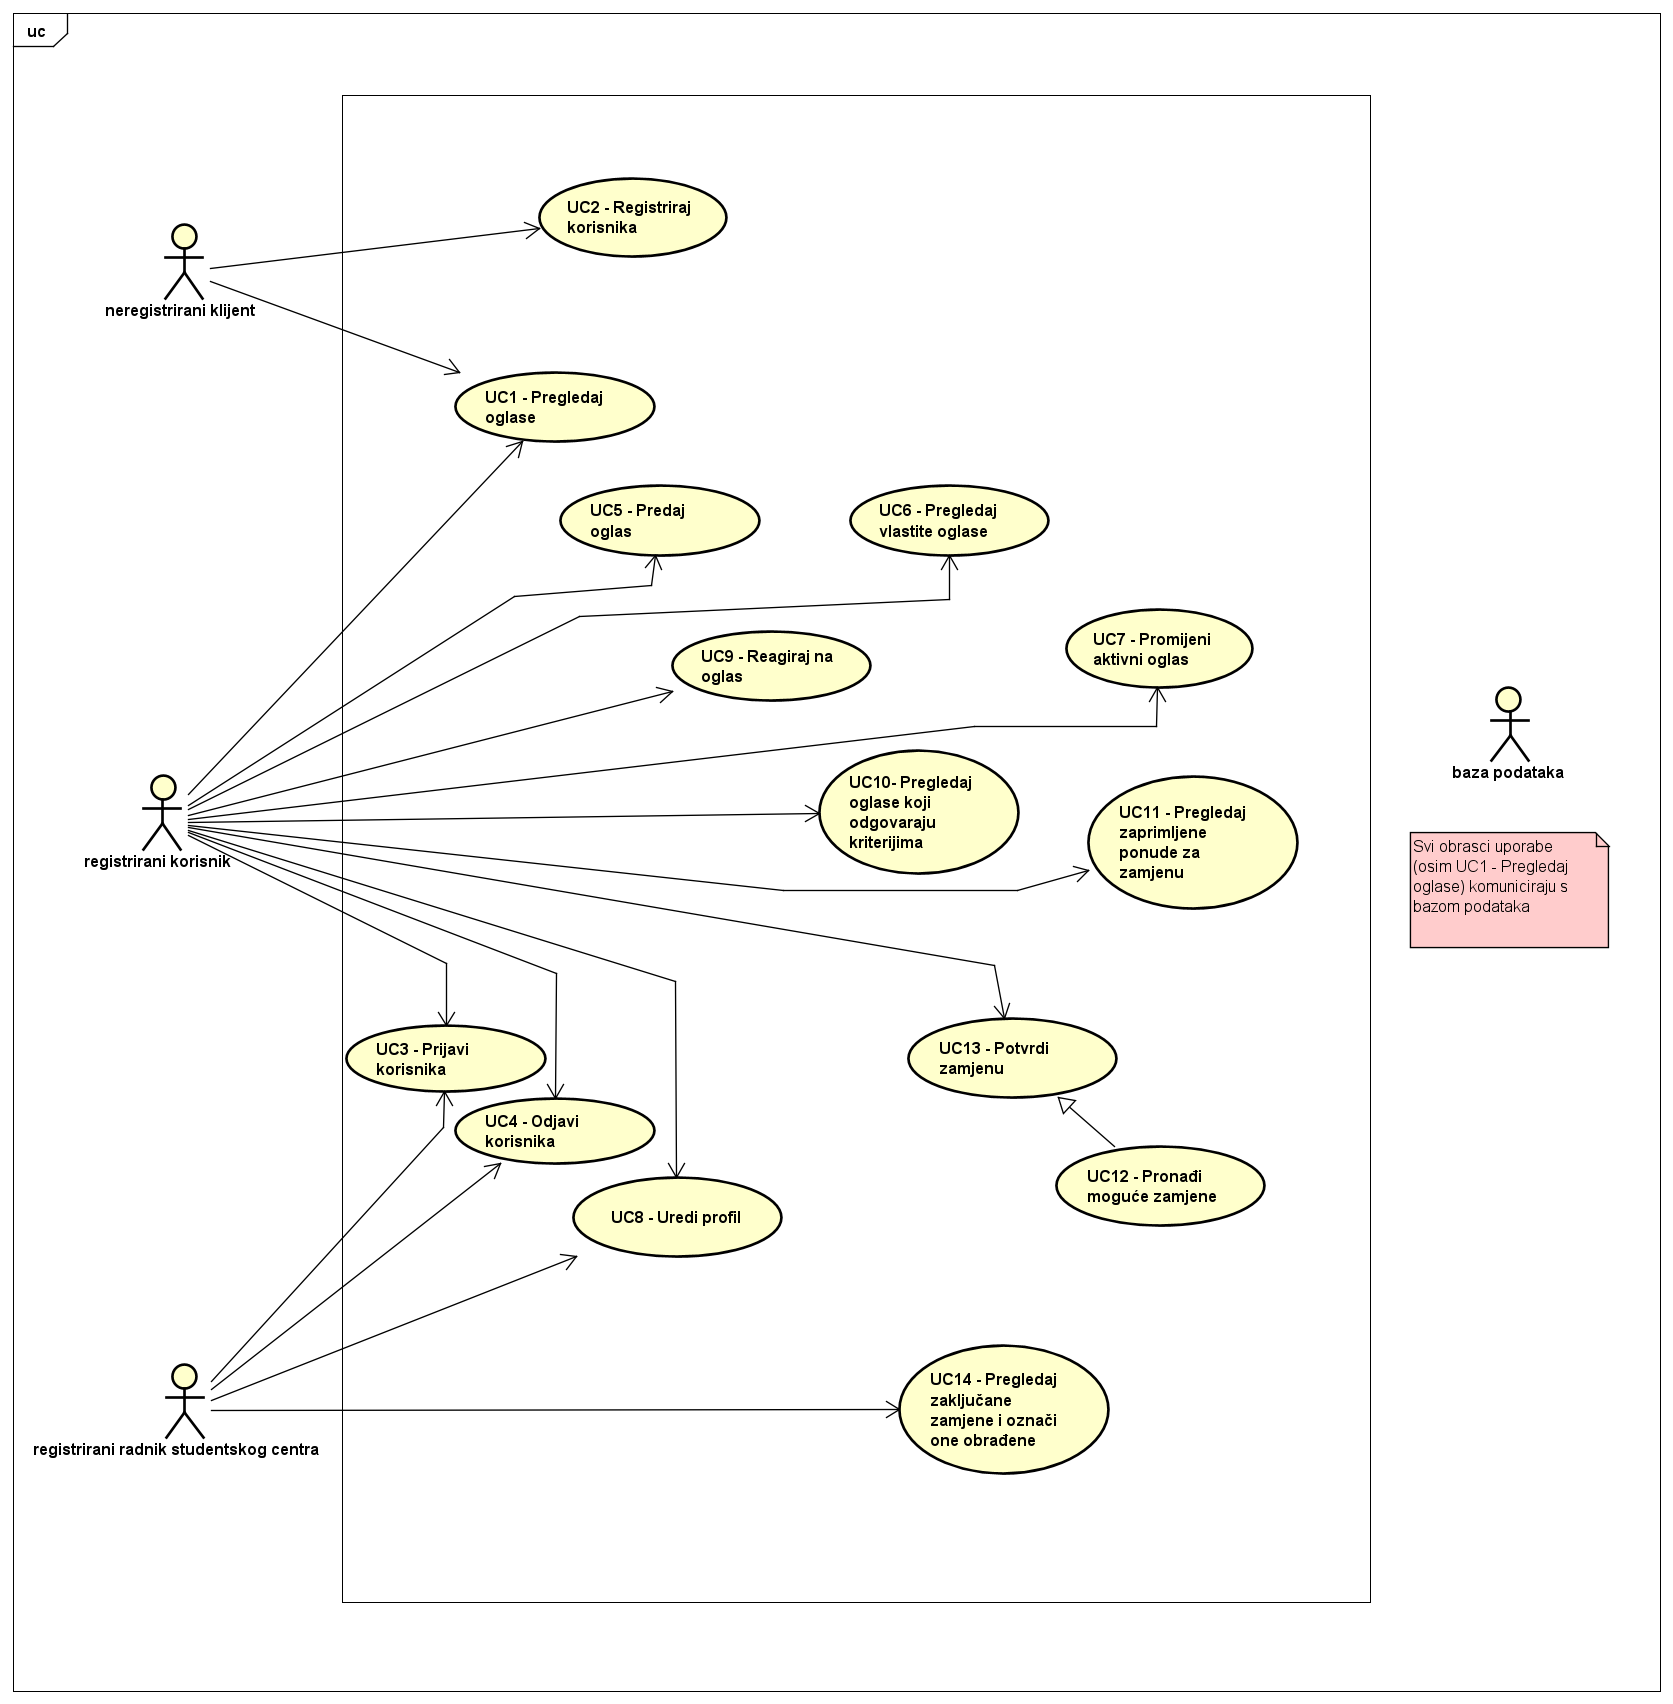
\includegraphics[width=.9\linewidth]{slike/UC_Diagram.PNG} %veličina u odnosu na širinu linije
	\centering
	\caption{Dijagram obrazaca uporabe}
	\label{fig:UC_Diagram} %label mora biti drugaciji za svaku sliku
\end{figure}

\eject	

\subsection{Sekvencijski dijagrami}
	
		\textbf{UC5 - Predaj oglas}
		\textit\\
		Registrirani korisnik šalje zahtjev za pregled vlastitih oglasa. Poslužitelj dohvaća korisnikove oglase iz baze podataka te ih prikazuje korisniku. Korisnik šalje zahtjev za stvaranje novog oglasa a poslužitelj mu vraća stranicu za stvaranje novog oglasa. Korisnik ispunjava novi oglas te šalje zahtjev za spremanje oglasa. Poslužitelj sprema oglas u bazu podataka i korisniku ispisuje poruku „Oglas uspješno predan“.

	
	\begin{figure}[H]
		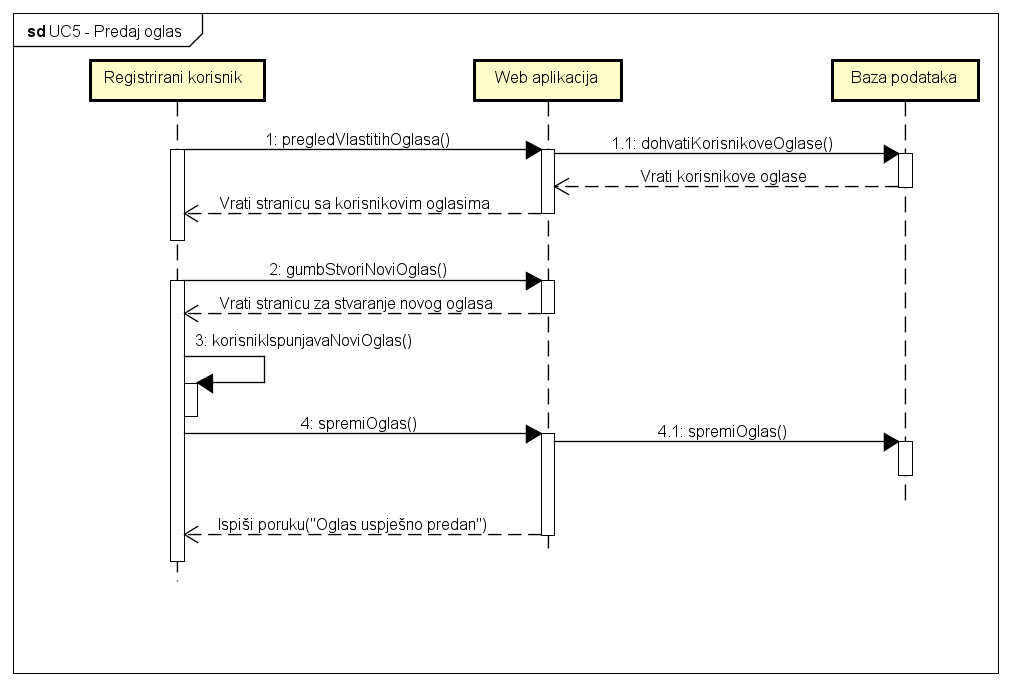
\includegraphics[width=.9\linewidth]{slike/UC5_sekvencijski_dijagram.PNG} %veličina u odnosu na širinu linije
		\centering
		\caption{Sekvencijski dijagram za UC5}
		\label{fig:sekvdij} %label mora biti drugaciji za svaku sliku
	\end{figure}

\eject
	
	\textbf{UC11 - Pregledaj zaprimljene ponude za zamjenu}
		\textit\\
		Registrirani korisnik šalje zahtjev za prikaz kandidata za zamjenu kako bi vidio oglase korisnika koji su  „lajkali“ njegov oglas i koji bi se htjeli zamjeniti za sobe sa njime. Poslužitelj dohvaća kandidate za zamjenu iz baze podataka i prikazuje ih korisniku. Ukoliko ne postoje kandidati za zamjenu poslužitelj prikazuje poruku  „Ne postoje kandidati za zamjenu“.  
		
	
	\begin{figure}[H]
		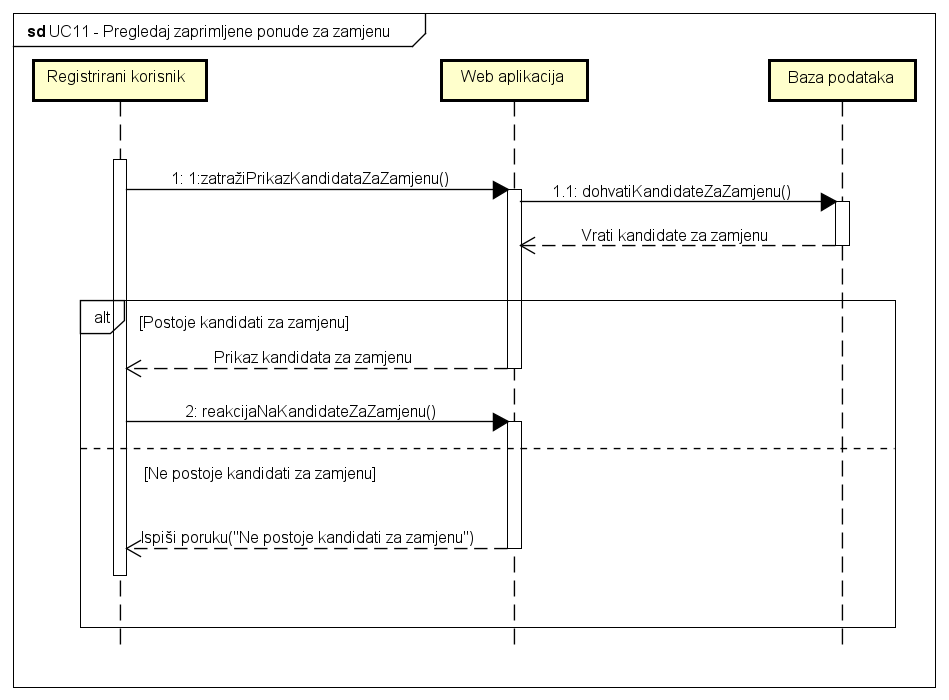
\includegraphics[width=.9\linewidth]{slike/UC11_sekvencijski_dijagram.PNG} %veličina u odnosu na širinu linije
		\centering
		\caption{Sekvencijski dijagram za UC11}
		\label{fig:sekvdij1} %label mora biti drugaciji za svaku sliku
	\end{figure}

\eject
	
		\textbf{UC13 - Potvrdi zamjenu}
		\textit\\
		Poslužitelj šalje korisniku e-mail za potvrdu zamjene. Registrirani korisnik klikne na link (odabere ga) te dolazi na web aplikaciju koja ga preusmjerava na stranicu za potvrdu. Korisnik potvrđuje ili odbija zamjenu, poslužitelj sprema promjenu u bazu podataka, te ako svi korisinici uključeni u zamjenu potvrde zamjenu poslužitelj ispisuje poruku „Zamjena potvrđena“, a ako jedan ili više korisnika uključenih u zamjenu odbiju zamjenu poslužitelj svim korisnicima uključenim u zamjenu ispisuje poruku „Zamjena odbijena“. Ukoliko prođe više od 7 dana te netko od korisnika ne potvrdi ili odbije zamjenu, poslužitelj briše podatke  o zamjeni iz baze podataka te korisnicima šalje e-mail o isteku ponude za zamjenu. 
		
	\begin{figure} [H]
		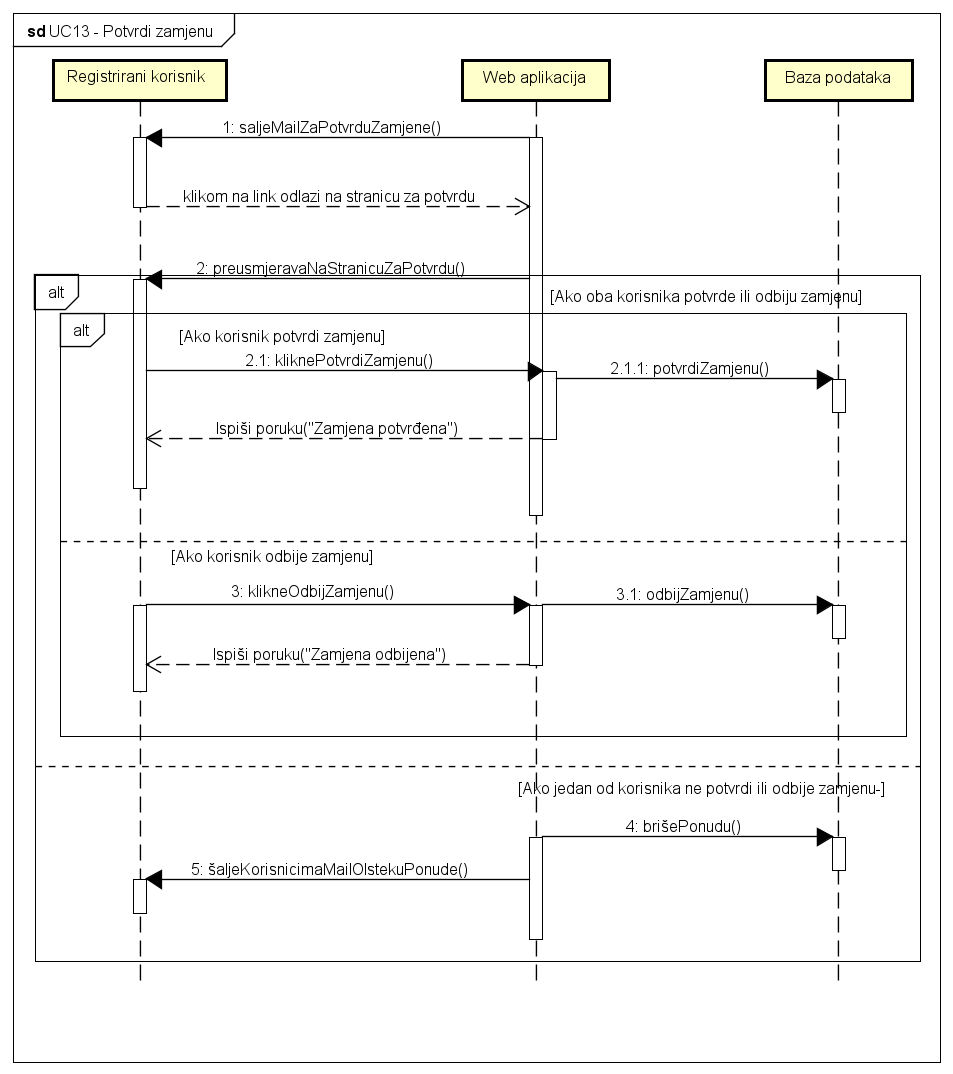
\includegraphics[width=.9\linewidth]{slike/UC13_sekvencijski_dijagram.PNG} 
		\centering
		\caption{Sekvencijski dijagram za UC13}
		\label{fig:sekvdij2}
	\end{figure}


\eject

\section{Ostali zahtjevi}

	\begin{itemize}
		\item 	\textit Sustav treba omoguciti rad više korisnika u stvarnom vremenu
		\item 	\textit Aplikacija treba biti prilagođena (engl. responsive) mobilnom uređaju
		\item 	\textit Korisničko sučelje i sustav moraju podržavati hrvatsku abecedu (dijakritičke znakove) prilikom unosa i prikaza tekstualnog sadržaja
		\item 	\textit Izvršavanje dijela programa u kojemu se pristupa bazi podataka ne smije trajati duže od nekoliko sekundi
		\item 	\textit Sustav treba biti implementiran kao web aplikacija koristeći objektrno-orijentirane jezike
		\item 	\textit Neispravno korištenje korisničkog sučelja ne smije narušiti funkcionalnost i rad sustava
		\item 	\textit Sustav treba biti jednostavan za korištenje, korisnici se moraju znati koristiti sučeljem bez opširnih uputa
		\item 	\textit Veza s bazom podataka mora biti kvalitetno zaštičena, brza i otporna na vanjske greške
		\item 	\textit Pristup sustavu mora biti omogućen iz javne mreže 
	\end{itemize}

